%\addcontentsline{toc}{chapter}{Development Process}
\chapter{Design}\label{chapt:design}

%You should concentrate on the more important aspects of the design. It is essential that an overview is presented before going into detail. As well as describing the design adopted it must also explain what other designs were considered and why they were rejected.

%The design should describe what you expected to do, and might also explain areas that you had to revise after some investigation.

%Typically, for an object-oriented design, the discussion will focus on the choice of objects and classes and the allocation of methods to classes. The use made of reusable components should be described and their source referenced. Particularly important decisions concerning data structures usually affect the architecture of a system and so should be described here.

%How much material you include on detailed design and implementation will depend very much on the nature of the project. It should not be padded out. Think about the significant aspects of your system. For example, describe the design of the user interface if it is a critical aspect of your system, or provide detail about methods and data structures that are not trivial. Do not spend time on long lists of trivial items and repetitive descriptions. If in doubt about what is appropriate, speak to your supervisor.

%You should also identify any support tools that you used. You should discuss your choice of implementation tools - programming language, compilers, database management system, program development environment, etc.

%Some example sub-sections may be as follows, but the specific sections are for you to define.

As the application was developed in an iterative manner, over a series of sprints, class diagrams and design diagrams were not created at the very start of the project. Instead, adopting an iterative approach to design was preferred. Regardless of this, some important design decisions were made at the start of the project. This chapter will clearly explain rationale for the decisions and state whether they were the result of an iterative processes or an upfront design.

\section{Overall architecture}
This section discusses the architecture of the web application. The design for the web application was developed over a series of sprints, iteratively increasing with each user story, therefore no upfront design was conducted at the start of the process.

\subsection{Class Diagram}
\label{architecture:class}
An overview of the resulting design of the class diagram is presented, with rationale for decisions made and how an iterative approach was used to reach the concluded design. The class diagram can be found in Appendix \ref{appendix:design}, section \ref{design:class_diagram}.

\subsubsection{Justification of design}
The following section discusses the appropriateness of the design and any justifications needed. Overall, the design clearly shows the object oriented principle of low coupling high cohesion being used on the project.

\noindent
\textbf{Google Services}
\newline
During early iterations, the Google Calendar API was only going to be utilised to parse the user's calendar events. As a result, the class \texttt{GoogleCalendarService} was created - this would ensure that the logic encapsulating the Google Calendar was centralised into one class. With the version number and API unlikely to change, constants were chosen as the best identifier; if the URLs and version number were to change in the future it would be easy to change these. The initial purpose of the class was to perform key operations to extract the events, as shown with the function \texttt{get\_events\_based\_on\_date}. The functions themselves were iteratively developed, initially only using the \texttt{execute\_request} and \texttt{get\_list\_of\_events}. Due to the scope changing with complexity, in the latter sprints  further functions were added.

Initially users were not considered a core part of the system. However, the user story to incorporate users into the system was created. Upon creation it was clear that another class to integrate with the Google Plus API would be required. This class followed a similar structure to the calendar class, except for parsing a user's email, so that it can be persisted in the database.

Eventually, the design was evaluated and duplicated functionality amongst the methods was discovered. In both of the classes the \texttt{build} and \texttt{execute\_request} functions were duplicated, without having class specific content. As a result, the extract class refactoring technique \cite{citeulike:14023810}, was used to create a super class \texttt{BaseGoogleService}. This class encapsulates logic for building  and executing queries. Extracting these functions to a super class ensured that pure logic for data and query manipulation can be moved to the \texttt{GoogleCalendarService} and \texttt{GooglePlusService} classes.


\noindent
\textbf{Helper classes}
\newline
Helper classes, in the design, are independent classes that help to modularise the system whilst grouping related functionality into a single class. As the system grew the duplication of code was beginning to become apparent, so helper classes aid in keeping a design simple.

For example the \texttt{SessionHelper} class was developed to initially store credentials after the oAuth log in, discussed in Section \ref{app:oauth}, had been completed and had successfully being appended to the session. The class' functions expanded as further duplication of the session handling was developed into the system.  This level of abstraction gave a semantic meaning to the interactions with the session.

Most of the helper classes do not interact with the other classes in the system. There is an exception with the \texttt{GoogleServicesHelper} class. In this class, majority of the functions are static. This design decision was induced due to the class not interacting with any specific class level attributes. Furthermore, prior to the implementation of editing a calendar event, the code was dispersed throughout the controllers. In an effort to reduce code duplication this helper class was created - but it was quickly decided that it would just be a proxy for calling specific functions in each of the services classes. Although ideally they should be class level functions, it is appropriate to use static functions.

\noindent
\textbf{Persistence classes}
\newline
The relationships between the persistence classes will not be discussed in this section (see Section \ref{section:er_diagram}). It is worth noting that designing the persistence classes was again an iterative process through the sprints. For example, for majority of the sprints the title attribute in the \texttt{NoteMetaData} class was not added. It wasn't until the a reflection on the content of a note was conducted that the design changed making this field a required attribute.

There are a series of \texttt{save} functions in the application and these were added to the design when the controllers were constantly duplicating functionality when persisting object to the database. This improved the readability of the application, providing a succinct solution to persisting an instance to the database.

In parts of the application, information needed to be extracted from the database. To aid in readability, static methods such as \texttt{find\_meta\_data} were created to keep domain related functionality together, but without creating a specific instance.

\noindent
\textbf{Binarisation}
\newline
The \texttt{BinariseImage} class is the model representation of the image segmentation script, as seen in section \ref{imp:image_proces}. The class is called from the controller when a user uploads their image. The output from the class methods is a binarised image. There are a series of functions which integrate with OpenCV API's \cite{citeulike:13206865}, manipulating an image and performing morphological operations. The class has been constructed so most of the functions are modular.

\subsection{CRC cards} \label{design:CRC}
To aid with the design, class collaboration cards (CRC) were drawn up for each feature. The user-story was decomposed into tasks and each of the tasks had associated CRC cards. This aided in thinking about the design for the class, as well as other classes it interacts with.  The overall design discussed in section \ref{architecture:class} is a result of the diligent planning with the CRC cards.

\begin{figure}[H]
  \centering
  \includegraphics[scale=0.5]{images/CRC_card}
  \caption{An example from Sprint 3, showing a CRC card at the very beginning of creation.}
  \label{fig:crc1}
\end{figure}

Figure \ref{fig:crc1} shows an example of a CRC card at the very beginning of the note class creation. The left hand side helped to think about methods and attributes for the class. The right hand side shows the responsibilities, where the note may interact with other classes.

Throughout each feature implemented into the system, the CRC cards were created, evaluated and refactored as ``throw away designs''. Although they were lightweight design tools, they helped to think about the system for the current feature being implemented - reducing the future design creep. For example, during the creation of the note into CRC cards, the image patch attribute was considered to be its own relation. After evaluating that this would be overcomplicating the design for the current feature this design decision was rejected and it would not add benefits to the existing system. The CRC cards were kept for each design and formulated into the class diagram at the end of the development process for formal documentation.

Overall CRC cards were at the forefront of the design during this project. They enabled a clear, concise and well considered design to evolve over a series of sprints. For a further example of an in-depth CRC card see, Appendix \ref{appendix:sup_design} section \ref{sup:crc}.

\subsection{User interaction} \label{design:user_interaction}
After deconstructing the problem that a user would need to be able to add a note, edit and save to a calendar, an activity diagram was constructed to consider the flow of the application.

Throughout the sprints, the design for the activity diagram expanded. The result is depicted in Figure \ref{fig:activity_show_note}. The user was not initially part of the application, so the activity did not include the first activity of logging into the system. This was included into diagram once the user story for users must be incorporated into the system was brought forward into the sprint.

\begin{figure}[H]
  \centering
  \includegraphics[scale=0.5]{images/saving_note_activity}
  \caption{An activity diagram to show how to save a note and the integrations with the calendar.}
  \label{fig:activity_show_note}
\end{figure}

The conditional checks to identify if there was meta-data outputted from the Tesseract output could not be clicked on to populate the form. This activity was included into the design during the planning of the feature for that sprint.

Overall, the activity diagram displayed shows the final output of how a note is added into the system. This design has been meticulously developed through a series of iterations to show the final output. It shows that a user can upload an image, they can select any associated meta-data from the suggestions, save the note and it will add it to the calendar item; there is also the option to edit the note.

\subsection{Model-view-controller}
The application would be designed in an Model-View-Controller (MVC) approach. Rationale for different aspects of the MVC structure will be discussed.

\subsubsection{About MVC}
MVC is a design pattern where logic is differentiated from presentation layers, as shown in Figure \ref{fig:mvc}.

The controller's aim is not to directly integrate with database and specific logic, instead to interact with a series of models and services. Finally, the controllers will aid in passing dynamic content to view files, returning rendered HTML.

The model in the MVC structure has no acknowledgement of the view file. Instead of rendering any form of HTML, the model is purely data-driven. The sole purpose of the model is to interact with the database and perform any business logic that does not fit in the controller and the view file.

Finally, the view files contain HTML logic with dynamic content passed from the controller. There may be specific logic which impacts the HTML displayed, but no direct calls are made to the database layer or the controller. It uses the dynamic content passed in.

\begin{figure}[H]
  \centering
  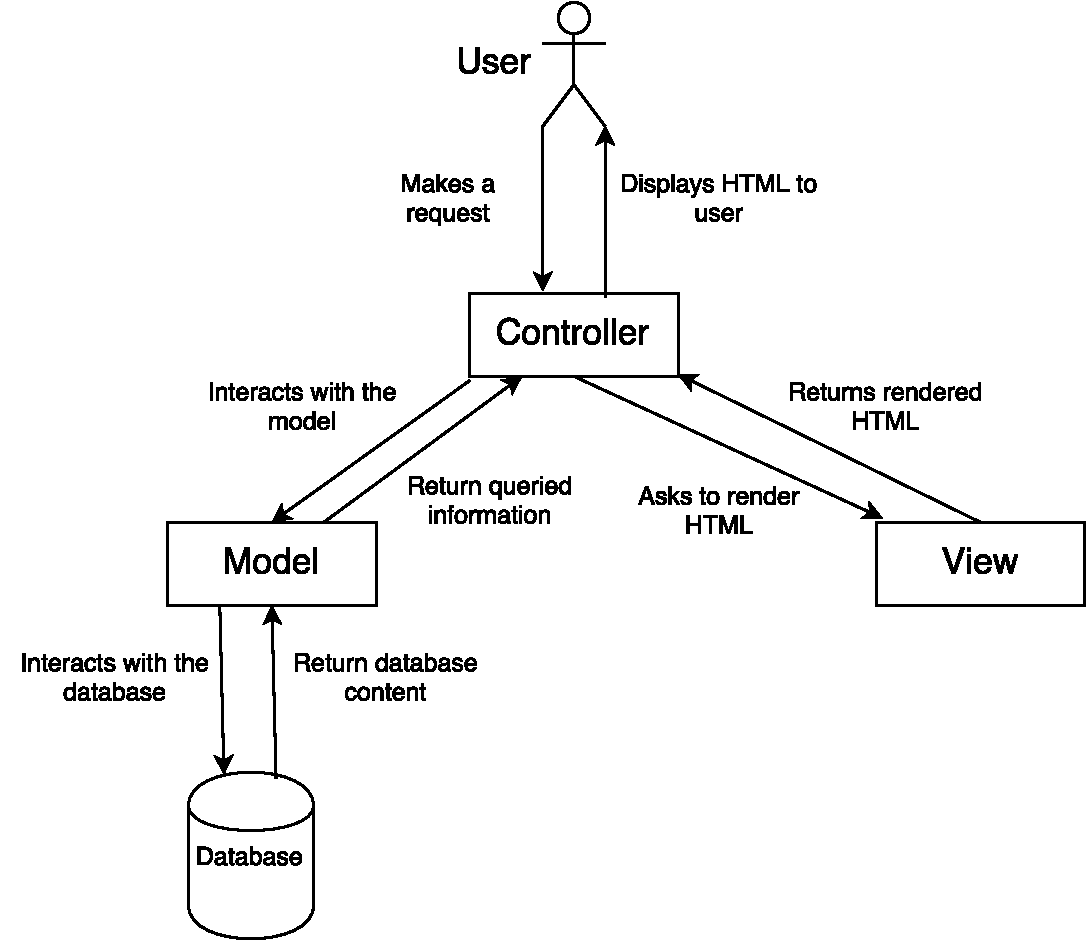
\includegraphics[scale=0.38]{images/MVC.pdf}
  \caption{A example of how the model-view-controller (MVC) framework integrates.}
  \label{fig:mvc}
\end{figure}

\subsubsection{Structuring the web application}
Although all the files could not be identified in the design section, the overall structure of the application has been considered.

The primary objective when considering the design of the application would be reusability of the codebase, where applicable. A module based design was considered, where each section of functionality was its own module - but this was rejected as it felt like the codebase would become obfuscated, due to related files - such as views - not being grouped together. Due to this preference an MVC approach would be appropriate as all the view files can be placed in the same directory.

The framework chosen (see Section \ref{language:framework}) does not support an MVC structure out of the box. Routes are expected to be placed in a singular file; this philosophy is carried through to the models. This was not chosen as the structure of the application as it reduces the clarity of the codes purpose. It also over-complicates the identification of interdependent classes, as it is not explicitly clear from the imports which class is used.

To overcome this, Blueprints \cite{citeulike:13983911} were used. Blueprints are modularised routes allowing different routing options to be placed in different files. Annotations were used to define the blueprint route - each being its own separate controller.

Models were separated into their own directory, and a one class per file policy was adopted to keep the design clean and simple. This ensured that the related file only represented the one class in the system - this would remove any ambiguity when looking at the directory structure.

It is worth considering the view files. The view files were the only section of the web application structure which underwent an iterative process. Initially, the view files would represent the entire document object model (DOM) in a singular file (duplicating headers, scripts etc). This is not the best design decision as there is core HTML which would not change between the different view files, so there was additional duplication that was redundant.

\begin{figure}[H]
  \centering
  \includegraphics[scale=0.5]{images/view_file_extension}
  \caption{A diagram illustrating how extension in Jinga html template engine works.}
  \label{fig:extension}
\end{figure}

Figure \ref{fig:extension} shows the result after the sprint which the design was improved upon. All template files now extend \texttt{root.html}, overriding the \texttt{content} block. This ensures that the Do not Repeat Yourself (DRY) principle is adhered to and HTML, such as the navigation, are only declared once.

\subsubsection{Constructing URLs} \label{design:urls}
Often overlooked when considering a design is the URL structure. The design not only aids the developer, but the user interacting with the page can clearly see the intention of that page. Typically there are two types of URLs - RESTful and query strings.

During the iterations, especially when new functionality was being considered, specific routes were thought about carefully. In the search user-story, query strings were preferred. Query strings create URLs such as: \texttt{/search?module\_code=cs31310}; representing the query string as key-value pairs. During the search feature, it was decided that this approach would be adopted so that the user can easily bookmark the page.

RESTful URLs help to show the a hierarchy of content. Exposing a user to such a URL helps them to clearly identify their content. When the system evolved to displaying a note for a user \texttt{/show\_note/1}, was chosen for the URL; it is easier to read than  \texttt{/show\_note?note\_id=1}. This allows the user to not have additional query parameters to decipher before working out the context of the page.

For the story of viewing notes, it was worth noting that traditional RESTful URLs would be adapted for readability. For example \texttt{/view\_notes/} was designed, when a proper RESTful URL may be \texttt{/notes/}. This offered more semantic meaning to the page's aim.

Overall the design considerations for the URL structure were an important design aspect that was considered to a great deal, to ensure that the user gets the best experience of interacting with the application as possible.

\section{Image processing}
In the very early sprints, the image processing design went through several substantial iterations. Each of the tasks relating to the user story to binarise an image had design implications.

Early work was conducted to investigate how to prepare images for the Tesseract engine. ImageMagick \cite{citeulike:14023816} was initially used by converting the image to greyscale - but this yielded poor results. After further design decisions were made to convert the image to monochrome this still returned too much noise. In the following iteration, the processing step would investigate whether the specific thresholding algorithms would be useful.
\begin{figure}[H]
  \centering
  
\includegraphics[scale=0.5]{images/image_binarisation_activity.pdf}
  \caption{An activity diagram to depict the design of the algorithm for the image segmentation.}
  \label{fig:activity_binarise}
\end{figure}

Figure \ref{fig:activity_binarise} shows the overall activity of how the image processing will be intended to be implemented, after early design work showed binarisation was more complex. Further descriptions of specific implementation can be found in the implementation section \ref{imp:image_proces}.

This high-level activity diagram shows the design stages which were used as a  high-level interpretation of the binarisation process. Initially a design was drawn up to just binarise the whole image, but due to implementation issues, this caused too much noise. Therefore, a new algorithm had to be established.

Blue lined paper was one way to overcome this issue. Filtering the lines from a thicker lined paper, would ensure less noise was on the image, creating a better binarised image. Overall, the activity diagram depicts the algorithm of taking a mobile phone photo, filtering the lines, binarising the image and extracting a tiff image. The tiff was selected as a design decision, as Tesseract input requires a tiff file.

This design initially considered blue lines to be important, but it was producing too much noise in the implementation. As a result, instead of trying to extract the lines, it was decided that the lines should be filtered and should only extract the text. This was the final iteration of development on the binarisation script.

\section{Tesseract} \label{design:tesseract}
During the analysis phase Tesseract was identified as the OCR tool of choice. Patel et al. \cite{citeulike:13920892} performed a case study using Tesseract as the OCR tool to analyse printed text in an image. Patel et al., also discuss the comparison against a proprietary OCR tool, Transym \cite{citeulike:14023819}.

Patel et al. concludes that Transym only yielded a 47\% accuracy on 20 images compared to 70\% accuracy using the Tesseract engine.

The first few iterations gave significant insight into how the document might be parsed. Due to the complexities with analysing the whole text on the image, it was limited to the first three lines, parsing the most useful information. It was decided that the first three lines were to be extracted forming the information for the metadata. Although design considerations for parsing the image and looking for key words was considered, it was ultimately rejected due to the complexity. Therefore, a structured approach was adopted. Below is an example of how the meta-data needs to be structured for the notes:

\begin{lstlisting}[caption={An example exert from a valid structured note}, label={lst:mock1}, breaklines, columns=fullflexible, basicstyle=\normalsize\ttfamily]
  CS31130: This is a title
  Date: 28th April 2016 14:00
  By: A Lecturer's name
\end{lstlisting}



It is worth acknowledging that the test-data used for the Tesseract training had a design element attached to it. When considering what the test data should consist of, there had to be a variety in the data. Training data drew from a range of textual resources ranging from  lecture notes \footnote{https://blackboard.aber.ac.uk/webapps/blackboard/content/listContent.jsp?course_id=_15108_1&content_id=_648523_1} to other objects such as mugs. Pangrams are a good way to represent text as it contains all alphabetical characters -  the ``quick brown fox'' is the most common example \cite{citeulike:14023830}. This would give Tesseract the best possible chance at learning different characters due to there being an abundance of each letter.

\section{Entity-relation design}\label{section:er_diagram}
Creating CRC cards enabled considerations to be made about the relations and how they are connected. Through each user-story analysed it was reflected upon and determined if it that would affect the entity-relation design.

\begin{figure}[H]
  \centering
  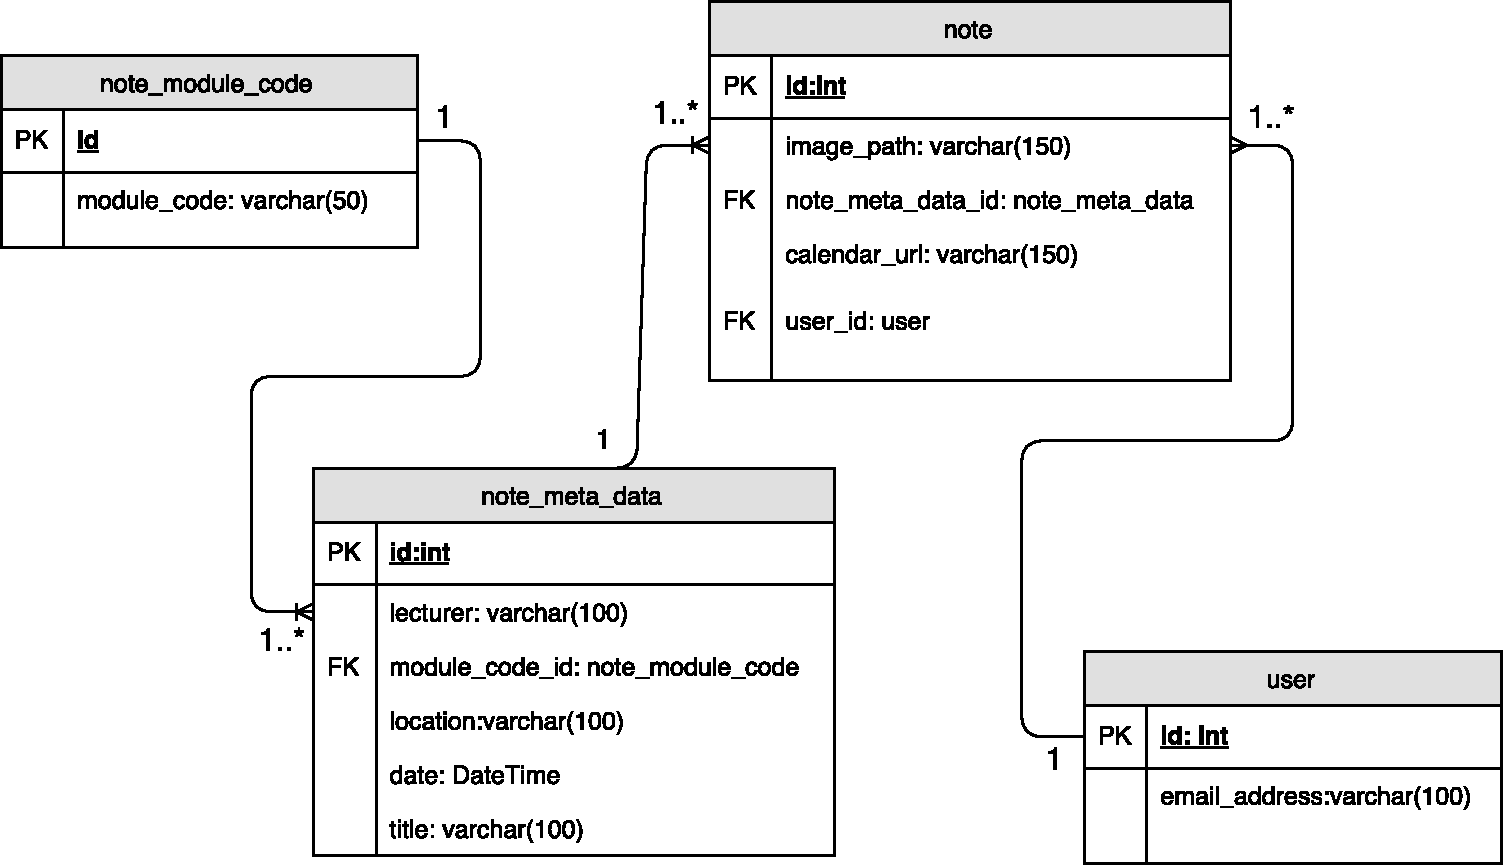
\includegraphics[scale=0.5]{images/database_diagram.pdf}
  \caption{The final result of the entity-relation diagram (after a series of iterations).}
  \label{fig:database}
\end{figure}

Figure \ref{fig:database}, shows the output from the result of the final design of the entity-relation diagram. Each new user story added new design implication to the design. For example, when the very basic user-story for creating a note was established, the metadata needed to be added in the future, but the story involved just a note. As a result just the image path attribute was added.

\subsection{Justification of design}
Below is a justification of the designs through various stories which affected the entity-relation design.

\noindent
\textbf{Note}
\newline
During design persisting the note was one of the first entity-relation design decisions which was made. The attributes selected for the \texttt{Note} relation best justify what is in a note. Firstly, the note contains an image link, which is a relative path to the image. This was persisted to ensure that it could be easily located. When the story for implementing users was actioned, an additional field containing the user's ID was added to the relation.

During the implementation of adding a URL to a calendar event, the calendar URL was persisted to the database of the associated note. The event ID could have be saved, but the URL was decided to persisted so additional queries were not made to the external service. Furthermore, a note will only have one URL.

When implementing the note's metadata, a relation was created and the foreign key was added to the note relation. This was created to ensure that a note must have associated metadata.

\noindent
\textbf{Note\_meta\_data}
\newline
The \texttt{note\_meta\_data} relation was created in its own relation to reduce data-redundancy, following the principle of normalisation in relational databases. The content could be duplicated for multiple notes if a user tags the same metadata to more than one note. As denoted from the relationships, a note will have a singular metadata item, but one metadata item could have many notes.

The attributes lecturer, location and datetime were the initially identified as part of the design decisions regarding what metadata should be saved. However, in a later iteration it was decided a title would be preferable; this was added to the relation. The date field is a date-time instead of a string due to integration with the calendar requires specific date-time strings, making it easier to parse.

Initially developed with the module code in this relation, in subsequent iterations the module code was extracted and a foreign key was used.

\noindent
\textbf{Module code}
\newline
The module code was developed into its own relation to prevent data-redundancy. A user may enter multiple notes for the same module code - as a result the database would only need to include one reference of that module code. The relationship between the metadata and the module code is explicit: the metadata must contain one module code but the module code can have more than one metadata item.

\noindent
\textbf{User}
\newline
This was not added to the application until around sprint five. However, the user will have an email address and that would be stored. It is in its own relation due to logic when creating a user: every time a user signs up to the system they are not creating a note instantly, therefore a relation was created to separate this logic. The foreign key was added to a note, so that a note can only have one user - and a user can have multiple notes.


\noindent
Overall, a succinct collection of relations have been developed which aim to solve the issues of data-redundancy, by providing solid rationale for the resulting design.


\section{User Interface}
As the web application was the main part of the project, a series of User Interface (UI) designs were collated at the start of each breakdown of the story.

The UI had to make the web application feel like an application, rather than a traditional website. This was identified from the background analysis where many systems felt like an application. The colour scheme was aiming to be simplistic, using the Google colour style guide \cite{citeulike:14023831}. An alternative of Bootstrap \cite{citeulike:13995818} was considered, instead of designing bespoke CSS. Although it has a built-in responsive theme, due to the overkill of the additional files, a simpler approach was adopted.

\begin{figure}[H]
  \centering
  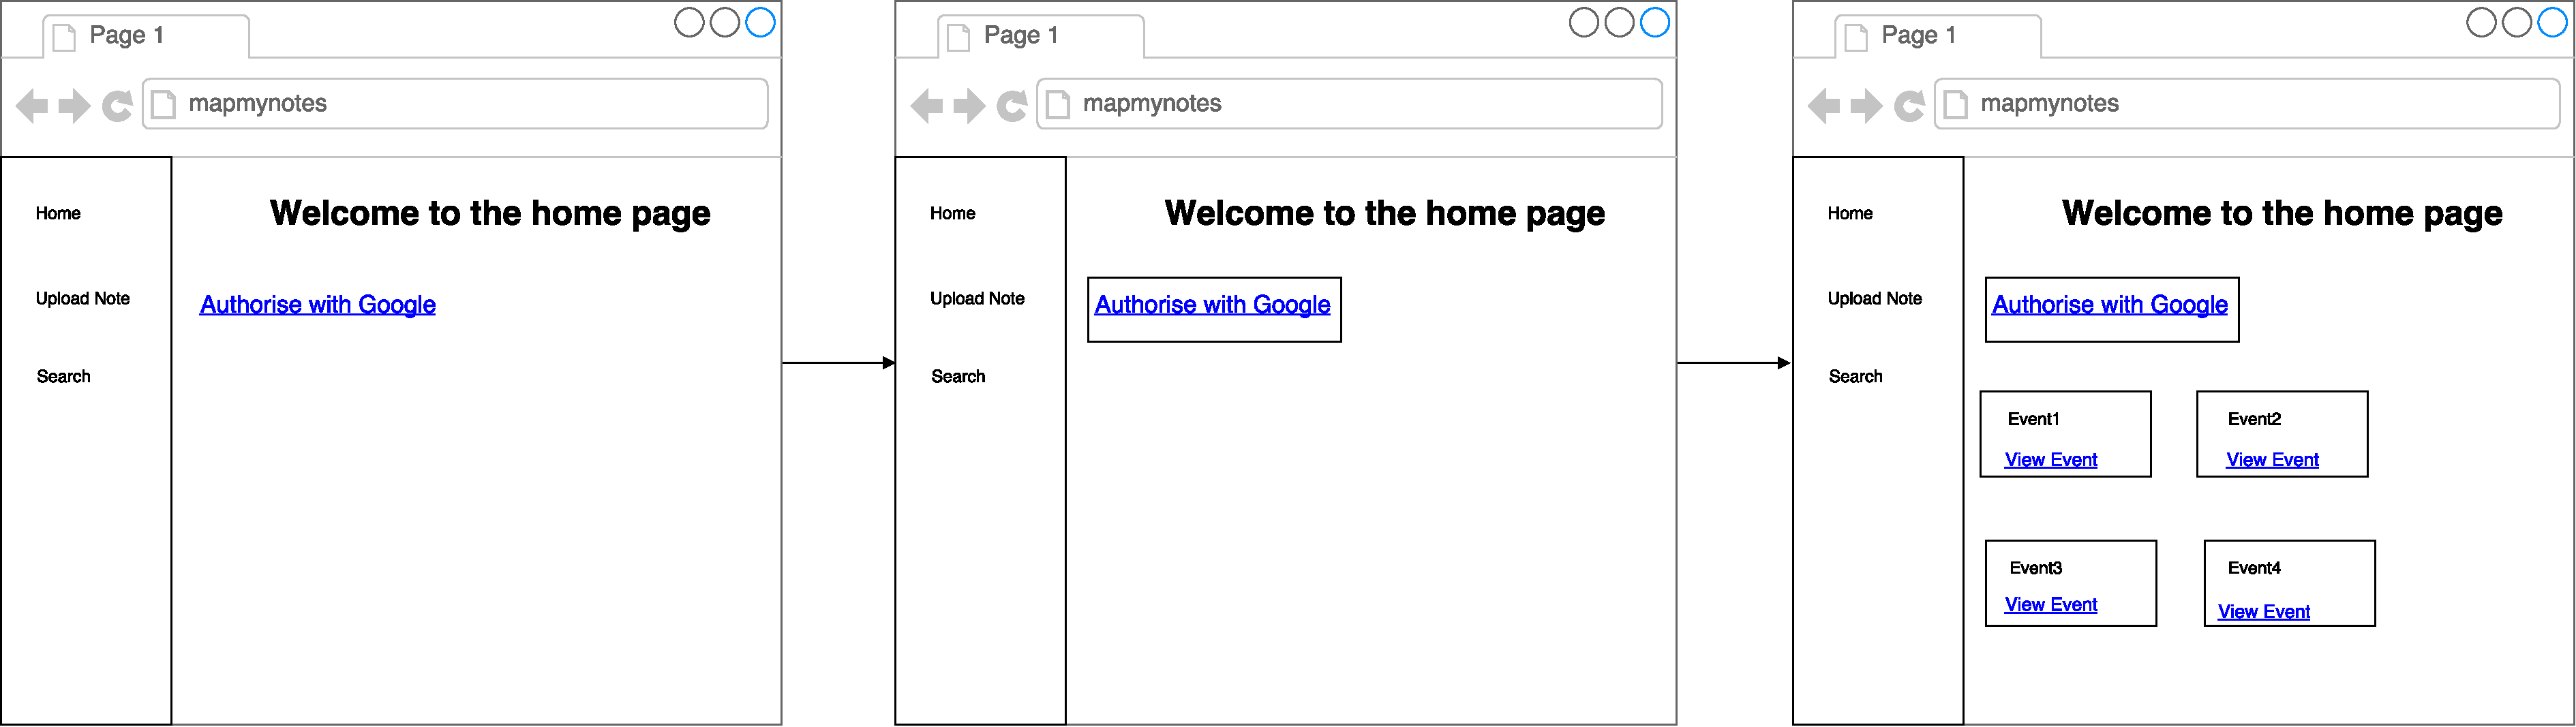
\includegraphics[scale=0.23]{images/homepage_wiremock.pdf}
  \caption{From left to right, the homepage wireframe through the different iterations and the change of requirements}
  \label{fig:homepage_wireframe}
\end{figure}

Figure \ref{fig:homepage_wireframe} shows the exploratory wireframe design completed prior to the UI. From the early iterations it was just an authorise button, then a requirement was added to show the user events from the last seven days where a wireframe was created to consider the design. This process was completed over the stories. If the story reflected a change in the content displayed on the screen, a conceptual design was mocked up to ensure there was an idea of how it intended to look.


Further mock-ups are available in Appendix \ref{appendix:sup_design}, Section \ref{sup:wireframe}.


\section{Implementation tools}
The following sections discuss the implementation tools and their purpose within the application.
\subsection{Programming language}
The programming language would not change per sprint or over an iterative process - as a result this was identified in sprint zero, when additional spike work was completed.

As a web application was being developed, investigatory work was completed into the suitability of several server-side languages. Traditionally server-side application languages are: PHP, Ruby, Python, C\#, Java and JavaScript, which has increased in popularity \cite{citeulike:14018462}.

Decomposition of the analysis in the early sprints determined that OpenCV would be utilised on the project. OpenCV's source code is written in C++, however Python and Java bindings are available. Additional research was conducted to see if a reliable wrapper for either PHP or Ruby was available, and after a lot of investigation it was concluded there was not.

C++ is not considered a standard web application development language,  therefore removing it as a viable option for the web application. Java applications are predominately large commercial applications, using a range of enterprise software - often renowned for their performance abilities \cite{citeulike:14019744}. This approach felt too cumbersome for a proposed light-weight application.

By being constrained by design decisions to use OpenCV and a reluctance to use Java, then Python was selected as the most suitable language. Python offers a lightweight and an easy to learn syntax that produces readable code, allowing a object-oriented paradigm to be followed. Additionally, its support for OpenCV is sufficient for the application.

\subsection{Framework} \label{language:framework}
As Python was being used as the language of choice, this narrowed down the frameworks available. Frameworks are useful for handling more complex features like routing and session handling - leaving the developer to focus on more domain specific issues.   Exploratory work was completed in the early sprints to find a suitable tool. Django \cite{citeulike:14019784}, Flask \cite{citeulike:13160396} and Bottle \cite{citeulike:14019792} were evaluated.

Frameworks can constrain the developers to specific implementations through abstracted classes whereas some offer more flexibility. Whilst evaluating Django, an extensive MVC framework, it was concluded that such a large tool was excessive for this application and it was rejected for the project.

Flask and Bottle are classified as `micro-frameworks', offering a lightweight structure, allowing developers to have more control over the structure. On face value, Flask and Bottle appear to be very similar; they are both lightweight with a similar syntax. After evaluating both of the frameworks it was concluded that Flask has a larger support community compared to Bottle, along with more reliable documentation.

As a result, Flask was chosen as the framework which will be used throughout the application. Spike work was completed into evaluating Flask's viability for the application quickly showed that it was a suitable tool.

\subsection{Continuous integration tools} \label{tools:CI}
Continuous Integration (CI) is normally used in development teams to ensure that all code is checked into the repository. As it was changed for a single person project, so did the point of using it; it was used to ensure every commit passed all tests when pushing to the repository.

After identifying CI would be used in the analysis stage, an appropriate tool would have to be chosen. Jenkins \cite{citeulike:14023837} was an initial choice; it is a standalone Java application to which a repository can be synced to.

Travis CI \cite{citeulike:14023840}, is a CI tool in the `cloud which can be synced to a GitHub repository. Tests can be run during every commit of the application and details regarding if it errors, passes or fails is available.

Although there was not much difference between the two tools, Travis did have the advantage that the web interface could be used rather than a standalone application. A disadvantage of Jenkins would be that for each branch, a built script would have to be developed. Ideally, the CI tool would be a quick set up and go process, not to be lumbered with further changes. As a result, Travis was chosen as the CI of choice.

\subsection{Version control}
Version control was used during the project so features could be worked on independently. The project was hosted in a private Git \cite{citeulike:14023846} repository on GitHub \cite{citeulike:13269771}. Git was chosen for its familiarity and GitHub is a well known place for handling Git based solutions; Travis CI integrated well with GitHub.

It is worth making a mention on the Git flow which was used. As each story was implemented a branch would be created in the form of: \texttt{feature/<summary\_of\_story>}, such as \texttt{feature/logout}. All branches were checked out from the development branch - ensuring that all features were from up to date commits. With each feature being developed in its own branch it ensured that any changes made would not affect the overall system. This provided a good platform to develop safely, whilst preserving working code.

Once the code was pushed to GitHub, Travis would automatically build the branch - inside the travis.yml file it would run a series of tests on the application. Once the tests had passed, a pull request would be made to merge the feature into the development branch. If this test successfully passes, and it is safe to merge, then it was merged to development.

\subsection{Development environment}
The text editor Atom \cite{citeulike:14023852} was used for the majority of the project. It is a lightweight text editor, which provides suitable syntax highlighting. However, later in the project when refactoring became more cumbersome due to the increase in code base - PyCharm community edition \cite{citeulike:14023855} was used as it offered better refactoring functionality.

\section{OAuth} \label{design:oauth}
Interactions with Google services would require the use of the OAuth2 protocol \cite{citeulike:11836766}. OAuth is a protocol which enables the authorisation and authentication of users to specific content.

From Google's comprehensive documentation on using OAuth2 \cite{citeulike:14026287} it was decided that `web application server` would be the most appropriate implementation.

When a user makes a request to the Google service it checks the authentication credentials, which are sent as part of the request, and authenticates the user. This checks to ensure that the email address and password are valid. If the user was to make another request to extract a list of events then the request would need to be authorised; a user may not be allowed to access specific content in the calendar, for example.

In the context of the application, a user will sign in with their Google credentials and Google will ask the user if they authorise the application to access their email address. Once authorised a \texttt{code} key is returned which is then subsequently used to exchange with the Google services. This code is then used to communicate to Google's service to returned a credential object, which contains an \texttt{Access Token} ID. This token ID is then used for all communication external services.

This was an enforced design as a result of using Google services, rather than any iterative approach.
